%!TEX root = ../main.tex
%%%%%%%%%%%%%%%%%%%%%%%%%%%%%%%%%%%%%
%
%LEZIONE 23/02/2016 - PRIMA SETTIMANA
%
%%%%%%%%%%%%%%%%%%%%%%%%%%%%%%%%%%%%%
\chapter{Calcolo in più dimensioni}
%%%%%%%%%%%%%
%CONTRAZIONI%
%%%%%%%%%%%%%
\section{Contrazioni}

\begin{teor}{Contrazioni}{contrazioni}\index{Contrazioni}
	Sia \(X\) uno spazio metrico completo e sia \(f\colon X\to X\) una mappa tale che
	\[
		\ex k\in[0,1):d\big(f(x),f(y)\big)\le k\,d(x,y),\,\fa x,y\in X,
	\]
	allora:
	\[
		\exists!\,\bar{x}\in X:f(\bar{x})=\bar{x}.
	\]
\end{teor}

\begin{proof}
	La strategia consiste nel dimostrare che \(f\) iterata in un punto è una successione di Cauchy, per poi dimostrare che, tramite la completezza, essa converge al punto fisso.
	Prima di mostrare ciò, andiamo a dimostrare le seguenti osservazioni:
	\begin{equation}\label{contr:1}
		d\big(f^n(x),f^n(y)\big)\le k^n d(x,y)
	\end{equation}
	ciò segue immediatamente dalla lipschitzianità di \(f\), infatti
	\[
		\begin{split}
			d\big(f^n(x),f^n(y)\big) & =d\big(f\circ f^{n-1}(x),f\circ f^{n-1}(y)\big)\\
			& \le k\,d\big(f^{n-1}(x),f^{n-1}(y)\big)\le\dots\graffito{itero il procedimento}\\
			& \le k^n d(x,y).
		\end{split}
	\]
	Verifichiamo inoltre che
	\begin{equation}\label{contr:2}
		d(x,y)\le\frac{1}{1-k}\Big[d\big(x,f(x)\big)+d\big(y,f(y)\big)\Big]
	\end{equation}
	infatti per la disuguaglianza triangolare si ha
	\[
		d(x,y)\le d\big(x,f(x)\big)+d\big(f(x),f(y)\big)+d\big(f(y),y\big),
	\]
	da cui applicando la lipschitzianità a \(d\big(f(x),f(y)\big)\) otteniamo
	\[
		d(x,y)\le d\big(x,f(x)\big)+k\,d(x,y)+d\big(f(y),y\big),
	\]
	da cui la \eqref{contr:2}.
	Osserviamo che l'ultima formula ci garantisce, se esiste, l'unicità del punto fisso.
	Infatti, se per assurdo tale punto non fosse unico, ovvero
	\[
		\ex\bar{x},\bar{y}\in X:f(\bar{x})=\bar{x}\text{ e }f(\bar{y})=\bar{y},
	\]
	si avrebbe
	\[
		d(\bar{x},\bar{y})\overset{\eqref{contr:2}}{\le}\frac{1}{1-k}\Big[d\big(\bar{x},f(\bar{x})\big)+d\big(\bar{y},f(\bar{y})\big)\Big],
	\]
	ovvero, per come sono stati presi \(\bar{x}\) ed \(\bar{y}\),
	\[
		d(\bar{x},\bar{y})\le\frac{1}{1-k}\Big[d\big(\bar{x},\bar{x}\big)+d\big(\bar{y},\bar{y}\big)\Big]=0,
	\]
	per cui \(\bar{x}=\bar{y}\).\\
	Mostriamo ora che, preso \(x_0\in X\), avremo che \(x_n=f^n(x_0)\) è una successione di Cauchy:
	\[
		\begin{split}
			d\big(f^n(x_0),f^m(x_0)\big) & \overset{\eqref{contr:2}}{\le}\frac{1}{1-k}\Big[d\big(f^n(x_0),f\circ f^n(x_0)\big)+d\big(f^m(x_0),f\circ f^m(x_0)\big)\Big]\\
			& \overset{\eqref{contr:1}}{\le}\frac{1}{1-k}\Big[k^n d\big(x_0,f(x_0)\big)+k^m d(x_0,f(x_0)\big)\Big]\\
			& =\frac{k^n+k^m}{1-k}d\big(x_0,f(x_0)\big)\xrightarrow{n,m}0,
		\end{split}
	\]
	quindi, per la completezza di \(X\), esisterà \(\bar{x}\in X\) tale che
	\[
		x_n\to\bar{x}.
	\]
	Dimostriamo infine che \(f(\bar{x})=\bar{x}\):
	\[
		\begin{split}
			d\big(\bar{x},f(\bar{x})\big) & =\graffito{ho potuto portare fuori il limite perchè sia \(f\) che \(d\) sono funzioni continue. \(f\) è continua perchè lipschitziana}\lim_{n\to+\infty}d\big(f^n(x_0),f\circ f^n(x_0)\big)\\
			& \overset{\eqref{contr:2}}{\le} k^n d\big(x_0,f(x_0)\big)\to 0,
		\end{split}
	\]
	ovvero
	\[
		\bar{x}=f(\bar{x}).\qedhere
	\]
\end{proof}

\begin{cor}
	Se \(x_0\in X\), allora
	\[
		f^n(x_0)\to\bar{x}.
	\]
\end{cor}

\begin{proof}
	Segue dalla dimostrazione del teorema.
\end{proof}

\begin{oss}
	In generale è quindi utile iterare la funzione contraente per ottenere il punto fisso.
\end{oss}

\begin{ese}
	Consideriamo la funzione \(f\colon\R\to\R,x\mapsto\frac{1}{2}x\), vogliamo mostrare che \(f\) è una contrazione di punto fisso nell'origine:
	\[
		\abs*{f(x),f(y)}=\abs*{\frac{1}{2}x-\frac{1}{2}y}=\frac{1}{2}\abs{x-y},
	\]
	pertanto \(f\) è per definizione una contrazione. Troviamo il suo punto fisso iterando la funzione:
	\[
		f(x) =\frac{1}{2}x,
	\]
	da cui
	\[
		f^2(x)=f\circ f(x)=\frac{1}{2}\frac{1}{2}x,
	\]
	ovvero, iterando
	\[
		f^n(x)=\left(\frac{1}{2}\right)^n x\to0,
	\]
	quindi, per il corollario del teorema delle contrazioni, l'origine è l'unico punto fisso di \(f\).
\end{ese}

\begin{oss}
	La figura \ref{fig:contr} mostra una rappresentazione geometrica del procedimento adottato.
\end{oss}

\begin{figure}[tp]
	\begin{centering}
		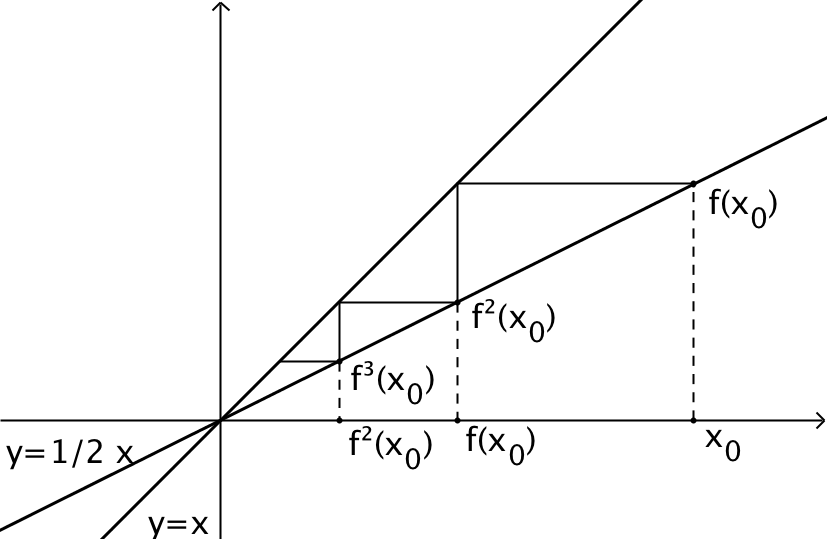
\includegraphics[height = 75mm]{fig1.png}
		\caption{La funzione \(\frac{1}{2}x\) iterata \(3\) volte.}
		\label{fig:contr}
	\end{centering}
\end{figure}

\begin{prop}{Distanza dal punto fisso}{distPuntoFisso}
	Sia \(X\) uno spazio metrico completo e sia \(f\colon X\to X\) una contrazione.
	Supponiamo che \(x_0\in X\) e che \(\bar{x}\in X\) sia il punto fisso di \(f\), allora:
	\[
		d\big(f^n(x_0),\bar{x}\big)\le\frac{k^n}{1-k}d\big(x_0,f(x_0)\big).
	\]
\end{prop}

\begin{proof}
	Sfruttando quanto visto nel teorema delle contrazioni (teorema \ref{th:contrazioni}) sappiamo che
	\[
		d\big(f^n(x_0),f^m(x_0)\big)\le\frac{k^n+k^m}{1-k}d\big(x_0,f(x_0)\big),
	\]
	passando al limite per \(m\to+\infty\) otteniamo
	\[
		d\big(f^n(x_0),\bar{x}\big)\le\frac{k^n}{1-k}d\big(x_0,f(x_0)\big).\qedhere
	\]
\end{proof}

\begin{cor}
	Se \(x_0\in X\), allora
	\[
		d(\bar{x},x_0)\le\frac{1}{1-k}d\big(x_0,f(x_0)\big).
	\]
\end{cor}

\begin{proof}
	Segue dalla proposizione, infatti
	\[
		\begin{split}
			d\big(f^n(x_0),\bar{x}\big) & \le\frac{k^n}{1-k}d\big(x_0,f(x_0)\big)\\
			& \le\frac{1}{1-k}d\big(x_0,f(x_0)\big).
		\end{split}
	\]
	Inoltre \(f^n(x_0)\to\bar{x}\), per cui
	\[
		d(\bar{x},x_0)\le\frac{1}{1-k}d\big(x_0,f(x_0)\big).\qedhere
	\]
\end{proof}

\begin{teor}{Contrazioni dipendenti da un parametro}{contrazioniDipPar}\index{Contrazioni!con parametro}
	Sia \(Y\) uno spazio metrico e sia \(X\) uno spazio metrico completo.
	Sia \(f\colon X\times Y\to X\) tale che:
	\begin{itemize}
		\item \(\ex k\in[0,1)\) tale che \(d_X\big(f(x,y),f(\tilde{x},y)\big)\le k\,d_X(x,\tilde{x})\), per ogni \(x,\tilde{x}\in X\);
		\item per ogni \(x\in X\) fissato, la mappa \(y\mapsto f(x,y)\) è continua.
	\end{itemize}
	Allora
	\[
		\fa y\in Y\,\exists!\,x(y):f\big(x(y),y\big)=x(y),
	\]
	inoltre la mappa
	\[
		y\mapsto x(y),
	\]
	è continua.
\end{teor}

\begin{proof}
	Per prima cosa mostriamo che \(f\) è continua in \((x,y)\).
	Sia \(d\) la distanza su \(X\times Y\), definita come
	\[
		d\big((x,y),(\tilde{x},\tilde{y})\big)=d_X(x,\tilde{x})+d_Y(y,\tilde{y}),
	\]
	la quale è facilmente verificabile essere una distanza.
	Prendiamo \((\tilde{x},\tilde{y})\) tali che
	\[
		d_X(x,\tilde{x})\le\frac{\e}{2 k},
	\]
	e
	\[
		d_Y(y,\tilde{y})\le\d_Y.
	\]
	Per la continuità di \(y\mapsto f(x,y)\), avremo
	\[
		\fa \e>0\,\ex \d_Y>0:d_Y(y,\tilde{y})<\d_Y\implies d_X\big(f(x,y),f(x,\tilde{y})\big)<\frac{\e}{2}.
	\]
	Quindi
	\[
		\begin{split}
			d_X\big(f(x,y),f(\tilde{x},\tilde{y})\big) & \le d_X\big(f(x,y),f(\tilde{x},y)\big)+d_X\big(f(\tilde{x},y),f(\tilde{x},\tilde{y})\big)\\
			& \le k \,d_X(x,\tilde{x})+\frac{\e}{2}\\
			& \le \frac{\e}{2}+\frac{\e}{2},
		\end{split}
	\]
	da cui la continuità di \(f\).\\
	Osserviamo che la mappa \(f_y: x\to f(x,y)\) è, per ipotesi, una contrazione, quindi, per il teorema \ref{th:contrazioni}
	\[
		\exists!\,x(y):f\big(x(y),y\big)=x(y).
	\]
	Dimostriamo la continuità in \(\bar{y}\), ovvero mostriamo che
	\[
		\fa\e>0\,\ex\d>0:d(y,\bar{y})<\d\implies d\big(x(y),x(\bar{y})\big)<\e.
	\]
	Per ogni \(y\) sia \(x(y)\) il punto fisso di \(f_y\), applicando la proposizione \ref{pr:distPuntoFisso} a \(d\big(x(y),x(\bar{y})\big)\), otteniamo:
	\[
		\begin{split}
			d\big(x(y),x(\bar{y})\big) & \le\frac{1}{1-k}d\big(f_y\big(x(\bar{y})\big),x(\bar{y})\big)\\
			& \le\graffito{applicando la disuguaglianza triangolare}\frac{1}{1-k}\Big[d\big(f_y\big(x(\bar{y})\big),f_{\bar{y}}\big(x(\bar{y})\big)\big)+\underbrace{d\big(f_{\bar{y}}\big(x(\bar{y})\big),x(\bar{y})\big)}_{=0}\Big]\\
			& =\frac{1}{1-k}d\big(f_y\big(x(\bar{y})\big),f_{\bar{y}}\big(x(\bar{y})\big)\big),
		\end{split}
	\]
	che è minore di \(\e\) quando \(d(y,\bar{y})<\d\) in quanto \(f\) è continua.
\end{proof}

\begin{defn}{Diffeomorfismo}{diffeomorfismo}\index{Diffeomorfismo}
	Sia \(D\subset\R^n\) un aperto.
	Una funzione \(f\colon D\to\R^n\) si definisce un \emph{diffeomorfismo} se è di classe \(C^1\), invertibile e la sua inversa è anch'essa di classe \(C^1\).
\end{defn}

\begin{teor}{di Inversione locale}{inversioneLocale}\index{Teorema!di inversione locale}
	Sia \(D\subset\R^n\) un aperto e sia \(f\colon D\to\R^n\) una funzione di classe \(C^1\).
	Supponiamo che per un \(x_0\in D,f'(x_0)\) sia invertibile, ovvero \(\det f'(x_0)\neq 0\), allora:
	\[
		\ex r>0:f|_{B_r(x_0)}
	\]
	è un diffeomorfismo sull'immagine.
\end{teor}

\begin{proof}
	Dobbiamo dimostrare che
	\[
		f\colon B_r(x_0)\to f\big(B_r(x_0)\big)
	\]
	è biiettiva e ha inversa di classe \(C^1\).

	Poniamo \(y_0=f(x_0)\), ci basta dimostrare che esiste
	\[
		g\colon f\big(B_r(x_0)\big)\to U_{x_0},\graffito{\(U_{x_0}\) indica un intorno di \(x_0\)}
	\]
	tale che \(g\) sia l'inversa di \(f\) su \(U_{x_0}\) e \(g(y_0+h)=g(y_0)+a(h)\), con
	\begin{equation}\label{eq:invLoc1}
		\norma{a(h)}\le C\norma{h},\,\fa h\text{ piccolo}.\tag{\(*\)}
	\end{equation}
	Se è vero ciò, \(g'(y_0)\) esiste e \(g'(y_0)=\big[f'(x_0)\big]^{-1}\).
	Mostriamo la validità di questa affermazione:
	\[
		f\big(g(y_0+h)\big)-f\big(g(y_0)\big)=y_0+h-y_0=h,
	\]
	in quanto \(g\) è l'inversa di \(f\), ma
	\[
		\begin{split}
			f\big(g(y_0+h)\big)-f\big(g(y_0)\big) & =f\big(g(y_0)+a(h)\big)-f\big(g(y_0)\big)\\
			& =f\big(x_0+a(h)\big)-f(x_0)\\
			& =f'(x_0)a(h)+o\big(\norma{a(h)}\big)\\
			& \overset{\eqref{eq:invLoc1}}{=}f'(x_0)a(h)+o\big(\norma{h}\big),
		\end{split}
	\]
	ovvero
	\[
		\begin{split}
			h=f'(x_0)a(h)+o\big(\norma{h}\big) & \iff f'(x_0)a(h)=h+o\big(\norma{h}\big)\\
			& \iff a(h)=\big[f'(x_0)\big]^{-1}h+o\big(\norma{h}\big),\graffito{poichè \(\big[f'(x_0)\big]^{-1}\) è una matrice costante}
		\end{split}
	\]
	da cui
	\[
		g(y_0+h)=g(y_0)+\big[f'(x_0)\big]^{-1}h+o\big(\norma{h}\big).
	\]
	Inizialmente abbiamo chiesto che \(\norma{a(h)}=O\big(\norma{h}\big)\), in realtà ci basta mostrare, affinchè valga \eqref{eq:invLoc1}, che
	\[
		\lim_{h\to0}a(h)=0,
	\]
	infatti, sappiamo che
	\[
		f\big(g(y_0+h)\big)-f\big(g(y_0)\big)=y_0+h-y_0=h,
	\]
	ma
	\[
		\begin{split}
			f\big(g(y_0+h)\big)-f\big(g(y_0)\big) & =f\big(x_0+a(h)\big)-f(x_0)\\
			& =f'(x_0)a(h)+o\big(\norma{a(h)}\big),
		\end{split}
	\]
	ovvero
	\[
		a(h)+o\big(\norma{a(h)}\big)=\big[f'(x_0)\big]^{-1}h,
	\]
	Poniamo \(k\big(a(h)\big)=o\big(\norma{a(h)}\big)\), da cui
	\[
		\lim_{h\to 0}\frac{\norma*{k\big(a(h)\big)}}{\norma{a(h)}}=0,
	\]
	ovvero \(\norma*{k\big(a(h)\big)}\le\frac{1}{2}\norma{a(h)}\) se \(\norma{h}\) è piccolo.
	Inoltre
	\[
		\norma*{a(h)+k\big(a(h)\big)}=\norma*{\big[f'(x_0)\big]^{-1}h},
	\]
	ma, applicando la triangolare inversa\graffito{\(\norma{a}\ge\big\lvert\norma{a+b}-\norma{b}\big\rvert\)}, si ottiene
	\[
		\begin{split}
			\norma*{a(h)+k\big(a(h)\big)} & \ge\norma{a(h)}-\norma*{k\big(a(h)\big)}\\
			& \ge\norma{a(h)}-\frac{1}{2}\norma{a(h)}\\
			& =\frac{1}{2}\norma{a(h)},
		\end{split}
	\]
	ovvero
	\[
		\begin{split}
			\frac{1}{2}\norma{a(h)} & \le\norma*{\big[f'(x_0)\big]^{-1}h}\\
			& \le\norma*{\big[f'(x_0)\big]^{-1}}_{op}\norma{h}\\
			& =C\norma{h},
		\end{split}
	\]
	che è proprio la \eqref{eq:invLoc1}.
	\begin{oss}
		La definizione di norma operatoriale per una matrice \(A\in M_{m,p}\) è
		\[
			\norma{A}_{op}=\sup_{\norma{x}=1}\norma{A\,x},
		\]
		dove \(\norma{A\,x}\le\norma{A}_{op}\norma{x}\).
	\end{oss}
	Affinchè valga \(a(h)\to 0\), ci basta mostrare che \(g\) è continua, in quanto
	\[
		g(y_0+h)=g(y_0)+a(h).
	\]
	La dimostrazione del teorema si riduce quindi alla ricerca di un'inversa continua \(g\).

	Definiamo
	\[
		H\colon D\times\R^n\to\R^n,(x,y)\mapsto x-f(x)+y,
	\]
	i punti fissi di \(H\) identificheranno le controimmagini di \(y\) tramite \(f\), infatti
	\[
		H(x,y)=x\iff x-f(x)+y=x,
	\]
	ovvero
	\[
		y=f(x).
	\]
	Cercheremo quindi di applicare il teorema delle contrazioni dipendenti da un parametro (\ref{th:contrazioniDipPar}) all'applicazione
	\[
		H\colon\overline{B_\d(x_0)}\times\overline{B_{\frac{\d}{2}}(y_0)}\to\overline{B_\d(x_0)}.
	\]
	Dimostrando che \(H\) è una contrazione in \(x\) uniforme in \(y\), otterremo che esiste un unico \(x\in\overline{B_\d(x_0)}\) tale che \(y=f(x)\).
	Dato \(y\in\overline{B_{\frac{\d}{2}}(y_0)}\) possiamo dunque trovare un \(x\in\overline{B_\d(x_0)}\) che risolve \(f(x)=y\).
	Se chiamiamo \(g\) l'applicazione che associa ad \(y\) tale \(x\), avremo
	\[
		f\big(g(y)\big)=y,
	\]
	e inoltre \(g\) sarà continua per il teorema.
	\begin{itemize}
		\item Mostriamo che \(H\) ha effettivamente \(\overline{B_\d(x_0)}\) come codominio:
		      \[
			      \begin{split}
				      \norma{H(x,y)-x_0} & =\norma{x-f(x)+y-x_0}\\
				      & =\norma*{(x-x_0)-\big[f(x)-f(x_0)\big]+(y-y_0)}\graffito{\(f(x_0)=y_0\)}\\
				      & \le\norma*{(x-x_0)-\big[f(x)-f(x_0)\big]}+\norma{y-y_0},
			      \end{split}
		      \]
		      posto \(\a\colon x\mapsto x-f(x)\), avremo
		      \[
			      \begin{split}
				      (x-x_0)-\big[f(x)-f(x_0)\big] & \mapsto\a(x)-\a(x_0)\\
				      & =\a'(x_0)(x-x_0)+o(x-x_0)\graffito{applicando Taylor}\\
				      & =o(x-x_0),
			      \end{split}
		      \]
		      in quanto \(\a'(x_0)=Id-Id\), per cui\graffito{vedi l'osservazione successiva per \(f'(x_0)=Id\)}
		      \[
			      \norma*{(x-x_0)-\big[f(x)-f(x_0)\big]}\le \norma{o(x-x_0)}\le\frac{1}{2}\norma{x-x_0}\le\frac{1}{2}\d.
		      \]
		      Infine \(y\in\overline{B_{\frac{\d}{2}}(y_0)}\) implica
		      \[
			      \norma{y-y_0}\le\frac{1}{2}\d,
		      \]
		      da cui
		      \[
			      \norma{H(x,y)-x_0}\le\d.
		      \]
		\item La continuità di \(y\mapsto H(x,y)\) è immediata dalla continuità di \(f\).
		\item Mostriamo che \(H\) è una contrazione in \(x\):
		      \[
			      \begin{split}
				      \norma{H(x,y)-H(x',y)} & =\norma*{\big[x-f(x)+y\big]-\big[x'-f(x')+y\big]}\\
				      & =\norma*{\big[x-f(x)\big]-\big[x'-f(x')\big]}\\
				      & \le\sup_{z\in\overline{B_\d(x_0)}}\norma{Id-f'(z)}_{op}\norma{x-x'}.
			      \end{split}
		      \]
		      Ora \(\norma{Id-f'(x_0)}_{op}=0\), per cui \(\norma{Id-f'(z)}_{op}\) è piccolo se \(z\in\overline{B_\d(x_0)}\) con \(\d\) opportuno.
		      Quindi \(\norma{Id-f'(z)}\le\frac{1}{2}\), da cui
		      \[
			      \norma{H(x,y)-H(x',y)}\le\frac{1}{2}\norma{x-x'}.
		      \]
	\end{itemize}
	\begin{oss}
		Possiamo sempre supporre che \(f'(x_0)=Id\).
		Infatti, se non lo fosse, possiamo definire
		\[
			\tilde{f}(x)=\big[f'(x_0)\big]^{-1}f(x),
		\]
		dove \(\tilde{f}'(x_0)=Id\).
		Una volta dimostrata l'invertibilità di \(\tilde{f}\), quella di \(f\) segue immediatamente da \(f(x)=\tilde{f}(x)f'(x_0)\).
	\end{oss}
	Abbiamo dunque dimostrato che esiste una \(g\) differenziabile tale che, se \(y\in B_{\frac{\d}{2}}(y_0)\), allora esiste unica \(g(y)\in B_\d(x_0):\big(f\circ g\big)(y)=y\).
	Per concludere il teorema devo dimostrare che
	\[
		g\big(B_{\frac{\d}{2}}(y_0)\big)\supseteq B_r(x_0),
	\]
	per qualche \(r>0\).
	Siccome \(f\) è continua, se \(r\) è piccolo, avremo
	\[
		f\big(B_r(x_0)\big)\subseteq B_{\frac{\d}{2}}(y_0),
	\]
	in tal caso \(g\) è definita su \(f\big(B_r(x_0)\big)\) e \(g\big(f(x)\big)=x\) per \(x\in B_r(x_0)\), ovvero
	\[
		B_r(x_0)\subseteq g\big(B_{\frac{\d}{2}}(y_0)\big).\qedhere
	\]
\end{proof}

\begin{cor}
	Se
	\[
		g\colon f\big(B_r(x_0)\big)\to B_r(x_0)
	\]
	è l'inversa di \(f\) e \(f(x_0)=y_0\), allora
	\[
		g'(y_0)=\big[f'(x_0)\big]^{-1}.
	\]
\end{cor}

\begin{oss}
	Il teorema è locale, ciò significa che l'inversa ha senso ed esiste solo tra intorni.
\end{oss}

\begin{oss}
	Se \(f\) non è di classe \(C^1\) il teorema è falso, mostriamolo con il seguente controesempio: consideriamo la bisettrice del piano, \(y=x\), e la parabola tangente ad essa nell'origine, \(y=\frac{1}{2}x^2+x\).
	Consideriamo quindi la funzione \(f\) della figura \ref{fig:invert}, tale funzione è differenziabile nell'origine in quanto è stretta da funzioni con derivata \(1\).
	Tale derivata non risulta però continua ed \(f\) non è iniettiva in un intorno dell'origine.
\end{oss}

\begin{figure}[htp]
	\begin{centering}
		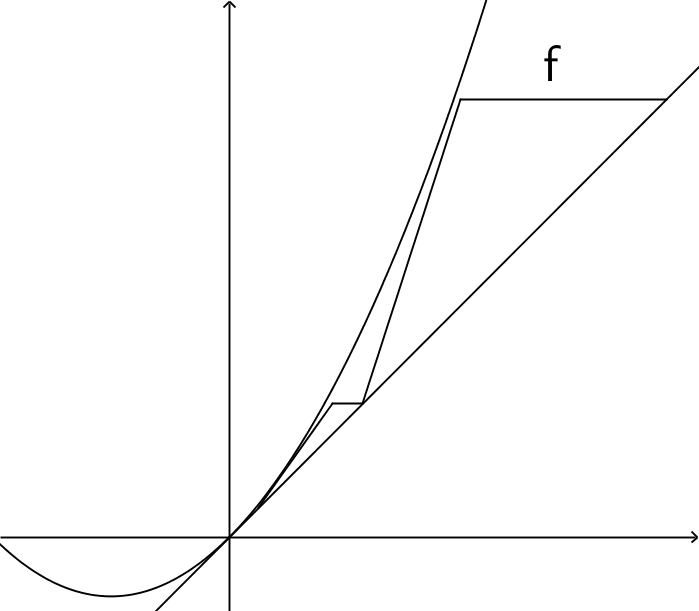
\includegraphics[height = 75mm]{fig2.png}
		\caption{La funzione \(f\) è stretta fra la parabola e la bisettrice.}
		\label{fig:invert}
	\end{centering}
\end{figure}

\begin{ese}
	Consideriamo la funzione delle coordinate polari
	\[
		f\colon S^1\times (0,+\infty)\to\R^2\setminus\{(0,0)\},(\q,\r)\mapsto(\r\cos\q,\r\sin\q),
	\]
	dove \(S^1=\frac{\R}{2\p\Z}\).
	Vogliamo mostrare che \(f\) ammette inversa di classe \(C^1\).

	Per applicare il teorema dobbiamo verificare che \(f\) sia invertibile di classe \(C^1\) e che \(f'\) sia localmente invertibile.
	\begin{itemize}
		\item Calcoliamo la jacobiana associata ad \(f\).
		      Abbiamo
		      \[
			      f\colon
			      \begin{pmatrix}
				      \q \\
				      \r
			      \end{pmatrix}
			      \mapsto
			      \begin{pmatrix}
				      x(\q,\r) \\
				      y(\q,\r)
			      \end{pmatrix}
			      ,\text{ con }
			      \begin{cases}
				      x(\q,\r)=\r\cos\q \\
				      y(\q,\r)=\r\sin\q
			      \end{cases}
			      ,
		      \]
		      da cui
		      \[
			      \begin{split}
				      f'
				      \begin{pmatrix}
					      \q \\
					      \r
				      \end{pmatrix}
				      & =
				      \begin{pmatrix}
					      \pd_\q x(\q,\r) & \pd_\r x(\q,\r) \\
					      \pd_\q y(\q,\r) & \pd_\r y(\q,\r)
				      \end{pmatrix}
				      \\
				      & =
				      \begin{pmatrix}
					      -\r\sin\q & \cos\q \\
					      \r\cos\q  & \sin\q
				      \end{pmatrix}
				      .
			      \end{split}
		      \]
		      Le derivate parziali di \(f\) sono visibilmente continue, per cui \(f\) è \(C^1\).
		\item Mostriamo che \(f\) è localmente invertibile:
		      supponiamo che \(f(\q,\r)=f(\q',\r')\), allora
		      \[
			      \begin{split}
				      \norma{f(\q,\r)}=\norma{f(\q',\r')} & \iff\norma{(\r\cos\q,\r\sin\q)}=\norma{(\r'\cos\q',\r'\sin\q')}\\
				      & \iff \sqrt{\r^2\cos^2\q+\r^2\sin^2\q}=\sqrt{{\r'}^2\cos^2\q'+{\r'}^2\sin^2\q'}\\
				      & \iff \r=\r',
			      \end{split}
		      \]
		      da cui
		      \[
			      \begin{split}
				      (\r\cos\q,\r\sin\q)=(\r\cos\q',\r\sin\q') & \iff (\cos\q,\sin\q)=(\cos\q',\sin\q')\\
				      & \iff \q-\q'\in2\p\Z\\
				      & \iff \q=\q',
			      \end{split}
		      \]
		      ovvero \(f\) è iniettiva.

		      La suriettività segue banalmente da
		      \[
			      \left(\arctan\frac{y}{x},\sqrt{x^2+y^2}\right)\mapsto (x,y),\,\fa x,y\in\R^2\setminus\{(0,0)\}.
		      \]
		\item Infine
		      \[
			      \det f'
			      \begin{pmatrix}
				      \r \\
				      \q
			      \end{pmatrix}
			      =-\r\neq 0,
		      \]
		      ovvero \(f'\) è localmente invertibile comunque presi \((\r,\q)\).
	\end{itemize}
	Quindi \(f\) è localmente invertibile con inversa di classe \(C^1\).
\end{ese}

\begin{ese}
	Un esempio analogo riguarda la funzione delle coordinate cilindriche
	\[
		f\colon (0,+\infty)\times S^1\times\R\to\R^3\setminus\{(0,0,0)\},
		\begin{pmatrix}
			\r \\
			\q \\
			\l
		\end{pmatrix}
		\mapsto
		\begin{pmatrix}
			\r\cos\q \\
			\r\sin\q \\
			\l
		\end{pmatrix}
		.
	\]
	Come nell'esercizio precedente si mostra facilmente che \(f\) è biiettiva di classe \(C^1\), per verificare che l'inversa è \(C^1\), è sufficiente dimostrare che \(\det f'\neq 0\).
	Calcoliamo quindi la jacobiana associata ad \(f\):
	\[
		f'
		\begin{pmatrix}
			\r \\
			\q \\
			\l
		\end{pmatrix}
		=
		\begin{pmatrix}
			\cos\q & -\r\sin\q & 0 \\
			\sin\q & \r\cos\q  & 0 \\
			0      & 0         & 1
		\end{pmatrix}
		,
	\]
	da cui
	\[
		\det f'
		\begin{pmatrix}
			\r \\
			\q \\
			\l
		\end{pmatrix}
		=\r\neq 0.
	\]
\end{ese}
%%%%%%%%%%%%%%%%%%%%%%%%%%%%%%%%%%%%%%%%%%%
%
%LEZIONE 01/03/2016 - SECONDA SETTIMANA (1)
%
%%%%%%%%%%%%%%%%%%%%%%%%%%%%%%%%%%%%%%%%%%%
%%%%%%%%%%%%%%%%%%%%%%%%%%%%%%%%%%
%TEOREMA DELLA FUNZIONE IMPLICITA%
%%%%%%%%%%%%%%%%%%%%%%%%%%%%%%%%%%
\section{Teorema della funzione implicita}

Lo scopo di questo paragrafo sarà stabilire se, presa una funzione
\[
	f(x,y)=0,
\]
è possibile esplicitare la variabile \(y\) in funzione della variabile \(x\).
Cercheremo inoltre di capire, nei casi in cui sarà possibile, quali sono le proprietà (continuità, differenziabilità) di \(y(x)\).

Cominciamo con l'analizzare alcuni esempi, nei quali tenteremo di capire sotto quali ipotesi è possibile esplicitare una variabile.

\begin{ese}
	Consideriamo la funzione \(f\colon\R^2\to\R,(x,y)\mapsto x^2+y^2-1\) e la curva
	\[
		\Set{(x,y)\in\R^2 | f(x,y)=0},
	\]
	rappresentata in figura \ref{fig:implicita1}.
	Naturalmente non è vero che, fissato \(x\), esiste un'unica \(y(x)\) che soddisfa l'equazione. Affinchè risulti vero, è necessario porsi in un intorno dove l'inversa sia locale.
	In tal caso troviamo un'unica \(y(x)\) che soddisfa l'equazione localmente.

	Ad esempio, se consideriamo il punto \(\left(\frac{1}{\sqrt{2}},\frac{1}{\sqrt{2}}\right)\), nell'intorno del semipiano superiore \(U=\Set{(x,y) | y>0}\), avremo
	\[
		y(x)=\sqrt{1-x^2}.
	\]
	Nello stesso modo potremmo esplicitare la \(x\) in funzione di \(y\) nell'intorno \(V=\Set{(x,y) | x>0}\), ottenendo
	\[
		x(y)=\sqrt{1-y^2}.
	\]
	Osserviamo che se invece considerassimo il punto \((0,1)\), non potremmo trovare un'unica \(x(y)\).
\end{ese}

\begin{figure}[tp]
	\begin{centering}
		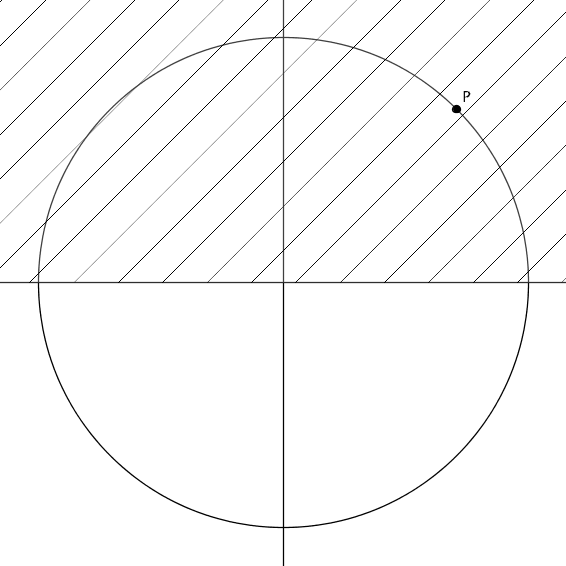
\includegraphics[height = 75mm]{implicita1.png}
		\caption{La circonferenza unitaria ristretta al semipiano superiore.}
		\label{fig:implicita1}
	\end{centering}
\end{figure}

\begin{ese}
	Consideriamo un esempio analogo in \(3\) dimensioni.
	Presa \(f\colon\R^3\to\R,(x,y,z)\mapsto x^2+y^2+z^2-1\), consideriamo la curva
	\[
		\Set{(x,y,z)\in\R^3 | f(x,y,z)=0},
	\]
	mostrata in figura \ref{fig:implicita2}.
	Se in questo caso consideriamo il punto \((0,0,1)\) nell'intorno \(U=\Set{(x,y,z) | z>0}\), possiamo esplicitare la \(z\) in funzione delle altre due variabili, ottendendo
	\[
		z(x,y)=\sqrt{1-x^2-y^2}.
	\]
	Questo procedimento non potrà mai essere applicato alle variabili \(x\) ed \(y\), in quanto ogni intorno del punto \((0,0,1)\) inconterà necessariamente due punti della curva.
\end{ese}

\begin{figure}[tp]
	\begin{centering}
		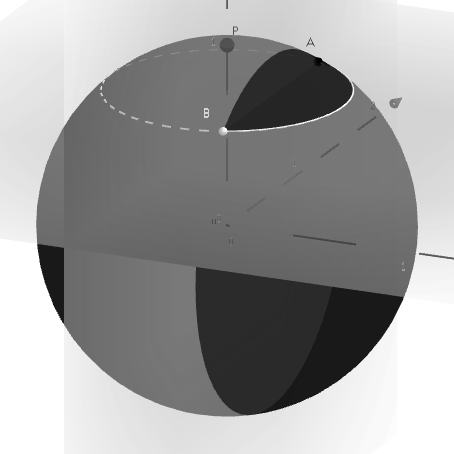
\includegraphics[height = 75mm]{implicita2.png}
		\caption{Nell'intorno di \((0,0,1)\), non è possibile esplicitare \(x\) o \(y\).}
		\label{fig:implicita2}
	\end{centering}
\end{figure}

\begin{ese}
	Consideriamo la funzione
	\[
		f\colon\R^3\to\R^2,
		\begin{pmatrix}
			x \\
			y \\
			z
		\end{pmatrix}
		\mapsto
		\begin{pmatrix}
			x^2+y^2+z^2-1 \\
			x^2+y^2-\frac{1}{2}
		\end{pmatrix}
		,
	\]
	associata alla curva
	\[
		\left\{
		\begin{pmatrix}
			x \\
			y \\
			z
		\end{pmatrix}
		:f(x,y,z)=0\right\}.
	\]
	Poniamoci in un intorno di \(\left(\frac{1}{2},\frac{1}{2},\frac{1}{\sqrt{2}}\right)\), ci aspettiamo di esplicitare due variabili in funzione della terza.

	Ad esempio, nell'intorno \(U=\Set{(x,y,z) | z>0,y>0}\) otteniamo, osservando che \(z\) può assumere soltanto il valore \(\frac{1}{\sqrt{2}}\),
	\[
		\begin{pmatrix}
			y(x) \\
			z(x)
		\end{pmatrix}
		=
		\begin{pmatrix}
			\sqrt{\frac{1}{2}-x^2} \\
			\frac{1}{\sqrt{2}}
		\end{pmatrix}
		.
	\]
	Analogamente, nell'intorno \(V=\Set{(x,y,z) | z>0,x>0}\), otteniamo
	\[
		\begin{pmatrix}
			x(x) \\
			z(x)
		\end{pmatrix}
		=
		\begin{pmatrix}
			\sqrt{\frac{1}{2}-y^2} \\
			\frac{1}{\sqrt{2}}
		\end{pmatrix}
		.
	\]
	Ovviamente non potremo esplicitare in funzione di \(z\), in quanto può assumere un unico valore, che va sempre ad identificare una circonferenza.
\end{ese}

\begin{oss}
	In generale vorremmo che, preso \(F\colon \R^m\times\R^n\to\R^n\), si abbia
	\[
		F\big(x,y(x)\big)=z_0,\,\fa x\in U_{x_0}.
	\]
	Ciò che faremo è applicare il teorema della funzione inversa, abbiamo quindi necessità di definire un'applicazione fra spazi uguali che ci aiuti nel nostro scopo.
	Consideriamo quindi
	\[
		G\colon\R^m\times\R^n\to\R^m\times\R^n,(x,y)\mapsto \big(x,F(x,y)\big).
	\]
	Supponiamo quindi che a \(G\) si possa applicare il teorema della funzione inversa, avremo quindi che
	\[
		G\colon U_{(x_0,y_0)}\to V_{\big(x_0,F(x_0,y_0)\big)},
	\]
	è invertibile, ovvero esiste
	\[
		G^{-1}\colon V_{\big(x_0,F(x_0,y_0)\big)}\to U_{(x_0,y_0)},(x,y)\mapsto\big(a(x,y),b(x,y)\big).
	\]
	Ora \(\big(G\circ G^{-1}\big)(x,y)=(x,y)\), da cui
	\[
		G\big(a(x,y),b(x,y)\big)=(x,y),
	\]
	ma
	\[
		G\big(a(x,y),b(x,y)\big)=\Big(a(x,y),F\big(a(x,y),b(x,y)\big)\Big).
	\]
	In particolare \(a(x,y)=x\), da cui
	\[
		\Big(x,F\big(x,b(x,y)\big)\Big)=(x,y),
	\]
	ovvero
	\[
		F\big(x,b(x,y)\big)=y.
	\]
	Quindi mi basta porre \(y(x)=b(x,z_0)\) per ottenere
	\[
		F\big(x,y(x)\big)=F\big(x,b(x,z_0)\big)=z_0,
	\]
	per ogni \(x\) in un intorno di \(X\).
\end{oss}

Siamo quindi pronti ad enunciare e dimostrare rigorosamente il teorema della funzione implicita.

\begin{teor}{della funzione implicita}{funzioneImplicita}\index{Teorema!della funzione implicita}
	Siano \(A\subseteq\R^m, B\subseteq \R^n\) due aperti.
	Sia \(f\colon A \times B \to \R^n\) di classe \(C^1\).
	Si supponga che \(f(x_0,y_0)=z_0\) e che \(\pd_y f(x_0,y_0)\) sia invertibile.

	Allora esiste un intorno \(U\) di \(x_0\), un intorno \(V\) di \(y_0\) e una funzione \(a\colon U \to V\) tale che
	\begin{itemize}
		\item Per ogni \(x\in U\), l'unica soluzione \(y\in V\) di \(f(x,y)=z_0\) è \(a(x)\);
		\item \(a\) è di classe \(C^1\) e vale
		      \[
			      a'(x_0) = -\big[\pd_y f|_{(x_0,y_0)}\big]^{-1} \pd_x f|_{(x_0,y_0)}.
		      \]
	\end{itemize}
\end{teor}

\begin{proof}
	Consideriamo la seguente funzione
	\[
		F \colon A \times B \to \R^m \times \R^n, \begin{pmatrix}x\\y\end{pmatrix} \mapsto 	\begin{pmatrix}
			x \\
			f(x,y)
		\end{pmatrix}.
	\]
	Tale funzione è di classe \(C^1\) in quanto \(f\) è \(C^1\) per ipotesi e \(y\) è banalmente \(C^1\).
	Inoltre vale
	\[
		F \begin{pmatrix}x_0\\y_0\end{pmatrix} = \begin{pmatrix}x_0\\z_0\end{pmatrix}
		\qquad\text{e}\qquad
		F' \begin{pmatrix}x_0\\y_0\end{pmatrix} = 	\begin{pmatrix}
			Id               & 0                \\
			\pd_x f(x_0,y_0) & \pd_y f(x_0,y_0)
		\end{pmatrix}.
	\]
	Mostriamo che \(F'(x_0,y_0)\) è invertibile.
	Fissato \((l,m)\) vogliamo quindi trovare \((h,k)\) tale che
	\[
		F' \begin{pmatrix}x_0\\y_0\end{pmatrix} \begin{pmatrix}h\\k\end{pmatrix} = \begin{pmatrix}l\\m\end{pmatrix},
	\]
	ovvero
	\[
		\begin{split}
			\begin{pmatrix}
				Id               & 0                \\
				\pd_x f(x_0,y_0) & \pd_y f(x_0,y_0)
			\end{pmatrix} \begin{pmatrix}h\\k\end{pmatrix} = \begin{pmatrix}l\\m\end{pmatrix} & \iff
			\begin{pmatrix}
				h \\
				\pd_x f(x_0,y_0)h + \pd_y f(x_0,y_0)k
			\end{pmatrix} = \begin{pmatrix}l\\m\end{pmatrix}\\
			& \iff 	\begin{cases}
				h = l \\
				\pd_x f(x_0,y_0)h + \pd_y f(x_0,y_0)k = m
			\end{cases}\\
			& \iff 	\begin{cases}
				h = l \\
				\pd_y f(x_0,y_0)k = m - \pd_x f(x_0,y_0)l
			\end{cases}\\
			& \iff 	\begin{cases}
				h = l \\
				k = \big[\pd_y f(x_0,y_0)\big]^{-1} \big(m - \pd_x f(x_0,y_0)l\big)\graffito{il passaggio è lecito in quanto \(\pd_y f(x_0,y_0)\) è invertibile per ipotesi}
			\end{cases}
		\end{split}
	\]
	Ci troviamo quindi nelle ipotesi del teorema della funzione inversa (\ref{th:inversioneLocale}).
	Per cui esistono degli intorni \(U_{(x_0,y_0)}\) e \(V_{(x_0,z_0)}\) in cui
	\[
		F\colon U_{(x_0,y_0)} \to V_{(x_0,z_0)},
	\]
	è invertibile tramite una funzione \(G\) di classe \(C^1\).

	La funzione \(G\) sarà del tipo
	\[
		G 	\begin{pmatrix}x\\y\end{pmatrix} = 	\begin{pmatrix}
			g(x,y) \\
			h(x,y)
		\end{pmatrix}.
	\]
	Per cui avremo
	\[
		(F\circ G) \begin{pmatrix}x\\y\end{pmatrix} = \begin{pmatrix}x\\y\end{pmatrix} \qquad\text{e}\qquad (F\circ G) \begin{pmatrix}x\\y\end{pmatrix} = F \begin{pmatrix}g(x,y)\\h(x,y)\end{pmatrix},
	\]
	da cui
	\[
		\begin{pmatrix}x\\y\end{pmatrix} = F \begin{pmatrix}g(x,y)\\h(x,y)\end{pmatrix} = 	\begin{pmatrix}
			x \\
			f \begin{pmatrix}g(x,y)\\h(x,y)\end{pmatrix}
		\end{pmatrix}.
	\]
	Da ciò segue, in particolare, che \(g(x,y)=x\), da cui
	\[
		\begin{cases}
			x = x \\
			y = f 	\begin{pmatrix}
				       x \\
				       h(x,y)
			       \end{pmatrix}
		\end{cases}
	\]
	A questo punto, è sufficiente porre
	\[
		a(x) = h(x,z_0),
	\]
	per ottenere che
	\[
		f\big(x,a(x)\big) = f\big(x,h(x,z_0)\big) = z_0.
	\]
	Dobbiamo ancora verificare che \(a\) sia definito in un intorno di \(x_0\), ma ciò segue dal fatto che \(a(x)=h(x,z_0)\) è definita come una componente di \(G\).
	Infatti
	\[
		G\colon V_{(x_0,z_0)} \to U_{(x_0,y_0)},
	\]
	dove, per la topologia prodotto
	\[
		V_{(x_0,z_0)} \supseteq B_r(x_0) \times B_r(z_0),
	\]
	quindi, in particolare
	\[
		x \in B_r(x_0),
	\]
	ovvero \(a\) è definito in un intorno di \(x_0\).

	Inoltre \(a\) è di classe \(C^1\) in quanto componente di \(G\) che è a sua volta \(C^1\).

	Resta da trovare la forma esplicita della derivata.
	Definiamo
	\[
		l\colon \R^m \to \R^m \times \R^n, x \mapsto \big(x,a(x)\big).
	\]
	Ora, se \(x\in B_r(x_0)\), avremo
	\[
		f\big(l(x)\big) = f\big(x,a(x)\big) \equiv z_0,
	\]
	da cui
	\[
		(f\circ l)'(x) = 0,\,\fa x \in B_r(x_0).
	\]
	Abbiamo
	\[
		f\circ l \colon \R^m \to \R^m \times \R^n \to \R^n,
	\]
	per cui \(f'\in M_{n \times (m+n)}\) e \(l'\in M_{(m+n)\times m}\).
	Inoltre
	\[
		f' \begin{pmatrix}x\\y\end{pmatrix} = \begin{pmatrix}\pd_x f(x,y) & \pd_y f(x,y)\end{pmatrix} \qquad\text{e}\qquad l'(x) = 	\begin{pmatrix}
			Id \\
			a'(x)
		\end{pmatrix}
	\]
	Da cui
	\[
		\begin{split}
			0 = (f\circ l)'(x_0) & = f'\big(l(x_0)\big)l'(x_0)\\
			& = \begin{pmatrix}\pd_x f(x,y) & \pd_y f(x,y)\end{pmatrix}|_{(x_0,a(x_0))} \begin{pmatrix}
				Id \\
				a'(x_0)
			\end{pmatrix}\graffito{\(\big(x_0,a(x_0)\big)=(x_0,y_0)\)}\\
			& = \pd_x f(x_0,y_0) + \pd_y f(x_0,y_0) a'(x_0),
		\end{split}
	\]
	ovvero
	\[
		a'(x_0) = -\big[\pd_y f(x_0,y_0)\big]^{-1} \pd_x f(x_0,y_0).\qedhere
	\]
\end{proof}

\begin{oss}
	In generale, preso \(y\in B_r(y_0)\), vale
	\[
		a'(y)=-\big[\pd_x f(a(y),y)\big]^{-1}\pd_y f(a(y),y).
	\]
\end{oss}

\begin{ese}
	Consideriamo nuovamente la funzione \(f\colon \R^2\to \R,(x,y)\mapsto x^2+y^2\), associata alla curva
	\[
		\Set{(x,y) | f(x,y)=1}.
	\]
	Questa volta, senza esplicitare realmente la \(y\), vogliamo trovare quanto vale la derivata della funzione, esplicitata in \(y\) rispetto ad \(x\), nel punto \((\frac{1}{\sqrt{2}},\frac{1}{\sqrt{2}})\).
	Verifichiamo per prima cosa che la derivata su \(y\) non sia nulla:
	\[
		\pd_y f\left(\frac{1}{\sqrt{2}},\frac{1}{\sqrt{2}}\right)=\frac{2}{\sqrt{2}}=\sqrt{2}\neq 0.
	\]
	Per il teorema, dal momento che \(f\) è chiaramente \(C^1\), avremo
	\[
		\begin{split}
			y'\left(\frac{1}{\sqrt{2}}\right) & =-\left[\pd_y f\left(\frac{1}{\sqrt{2}}\right)\right]^{-1}\pd_x f\left(\frac{1}{\sqrt{2}}\right)\\
			& =-\frac{1}{\sqrt{2}}\sqrt{2}\\
			& =-1.
		\end{split}
	\]
\end{ese}

\begin{ese}
	Consideriamo la funzione
	\[
		F\colon\R^3\to\R^2,
		\begin{pmatrix}
			x \\
			y \\
			z
		\end{pmatrix}
		\to
		\begin{pmatrix}
			x^2+y^2+z^2 \\
			x^2+y^2
		\end{pmatrix}
		,
	\]
	associata alla curva
	\[
		\Set{(x,y,z) | F
			\begin{pmatrix}
				x \\
				y \\
				z
			\end{pmatrix}
			=
			\begin{pmatrix}
				1 \\
				\frac{1}{2}
			\end{pmatrix}
		}.
	\]
	Verifichiamo se è possibile applicare il teorema al punto \((\frac{1}{2},\frac{1}{2},\frac{1}{\sqrt{2}})\), esplicitando \(y\) e \(z\) rispetto ad \(x\).
	\[
		\begin{split}
			\pd_{y,z}F\left(\frac{1}{2},\frac{1}{2},\frac{1}{\sqrt{2}}\right) & =
			\begin{pmatrix}
				2y & 2z \\
				2y & 0
			\end{pmatrix}_{(\frac{1}{2},\frac{1}{2},\frac{1}{\sqrt{2}})}
			\\
			& =
			\begin{pmatrix}
				1 & \sqrt{2} \\
				1 & 0
			\end{pmatrix}
			\\
			& \neq 0.
		\end{split}
	\]
	per cui \(\pd_{y,z}F\) è invertibile, posso quindi applicare il teorema.
	Avremo
	\[
		\begin{split}
			\begin{pmatrix}
				y'\left(\frac{1}{2}\right) \\
				z'\left(\frac{1}{2}\right)
			\end{pmatrix}
			& =-\left[\pd_{y,z}F\left(\frac{1}{2},\frac{1}{2},\frac{1}{\sqrt{2}}\right)\right]^{-1}\pd_x F\left(\frac{1}{2},\frac{1}{2},\frac{1}{\sqrt{2}}\right)\\
			& =-
			\begin{pmatrix}
				1 & \sqrt{2} \\
				1 & 0
			\end{pmatrix}^{-1}
			\begin{pmatrix}
				1 \\
				1
			\end{pmatrix}
			,
		\end{split}
	\]
	dove
	\[
		\begin{split}
			\begin{pmatrix}
				1 & \sqrt{2} \\
				1 & 0
			\end{pmatrix}^{-1}
			& =-\frac{1}{\sqrt{2}}
			^{t}\begin{pmatrix}
				0         & -1 \\
				-\sqrt{2} & 1
			\end{pmatrix}
			\\
			& =-\frac{1}{\sqrt{2}}
			\begin{pmatrix}
				0  & -\sqrt{2} \\
				-1 & 1
			\end{pmatrix}
			\\
			& =
			\begin{pmatrix}
				0                  & 1                   \\
				\frac{1}{\sqrt{2}} & -\frac{1}{\sqrt{2}}
			\end{pmatrix}
			,
		\end{split}
	\]
	da cui
	\[
		\begin{pmatrix}
			y'\left(\frac{1}{2}\right) \\
			z'\left(\frac{1}{2}\right)
		\end{pmatrix}
		=-
		\begin{pmatrix}
			0                  & 1                   \\
			\frac{1}{\sqrt{2}} & -\frac{1}{\sqrt{2}}
		\end{pmatrix}
		\begin{pmatrix}
			1 \\
			1
		\end{pmatrix}
		=
		\begin{pmatrix}
			-1 \\
			0
		\end{pmatrix}
		.
	\]
\end{ese}
%%%%%%%%%%%%%%%%%%%%%%%%%%%%%%%%%%%%%%%%%%%
%
%LEZIONE 02/03/2016 - SECONDA SETTIMANA (2)
%
%%%%%%%%%%%%%%%%%%%%%%%%%%%%%%%%%%%%%%%%%%%
%%%%%%%%%%%%%%%%%%%%%%%%%%%%
%MOLTIPLICATORI DI LAGRANGE%
%%%%%%%%%%%%%%%%%%%%%%%%%%%%
\section{Moltiplicatori di Lagrange}

In questo paragrafo studieremo un metodo pratico per la ricerca di massimi e minimi vincolati.
Per farlo introdurremo i concetti di \emph{curve di livello} e di \emph{moltiplicatori di Lagrange}.
Come prima cosa mostriamo un esempio tipico, risolubile anche a mano, che ci mostra il genere di problemi che studieremo.

\begin{ese}
	Supponiamo di voler massimizzare \(x+y\) sotto il vincolo \(x^2+y^2=1\).
	In questo caso la funzione da massimizzare rappresenta tutte le rette del piano di pendenza \(-1\), mentre il vincolo è costituito dalla circonferenza unitaria.
	Come è evidente dalla figura \ref{fig:molt1} il massimo è raggiunto nel punto \(P=(1/\sqrt{2},1/\sqrt{2})\) con \(f(P)=\sqrt{2}\).
	Osserviamo che le linee di livello di \(x+y\) raggiungono il massimo, rispetto al vincolo, nel punto di tangenza alla circonferenza, osserveremo questo comportamento anche in seguito.
\end{ese}

\begin{figure}[tp]
	\begin{centering}
		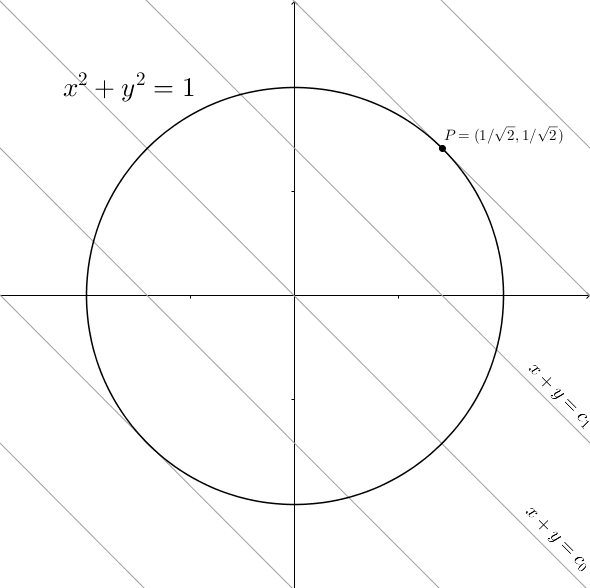
\includegraphics[height = 75mm]{molt1.png}
		\caption{La funzione \(x+y\) e il suo vincolo sul piano \(\R^2\).}
		\label{fig:molt1}
	\end{centering}
\end{figure}

\begin{notz}
	Da questo momento, presa una funzione \(f\colon \R^n\to \R\), utilizzaremo il simbolo \(f'(x)\) per fare riferimeno al vettore riga delle dereivate parziali di \(f\), mentre useremo il simbolo di \emph{nabla} \(\nabla f(x)\), per far riferimento al vettore colonna delle derivate parziali.
\end{notz}

\begin{oss}
	Questo uso arbitrario di vettori riga o colonna può essere giustificato rigorosamente tramite il ben noto isomorfismo \(\R^n\simeq\big(\R^n\big)^*\).
	Infatti, se consideriamo \(f\colon\R^n\to\R\) avremo che
	\[
		f'(x)\in M_{1,n}(\R),
	\]
	la quale, in vista della corrispondenza biunivoca fra matrici \(n\times m\) e applicazioni lineari da \(\R^m\) in \(\R^n\), può essere associata ad un'applicazione lineare da \(\R^n\) in \(\R\), ovvero ad un elemento del duale di \(\R^n\).
	In virtù del suddetto isomorfismo, esisterà
	\[
		\j:\big(\R^n\big)^*\to\R^n,(x_1,\dots,x_n)\mapsto
		\begin{pmatrix}
			x_1   \\
			\dots \\
			x_n
		\end{pmatrix}
	\]
	ed è tale che vale
	\[
		\big(\j(x),y\big)={}^{t}x\,y,
	\]
	per cui
	\[
		\nabla f(x)={}^{t}\big(f'(x)\big)=\j\big(f'(x)\big).
	\]
\end{oss}

\begin{defn}{Linee di livello}{lineeLivello}\index{Linee di livello}
	Consideriamo una funzione \(f\colon A\subset\R^n\to \R\) e \(c_n\in\R\).
	Si definisce \emph{curva di livello} l'insieme costituito dai punti di \(A\) che soddisfano l'equazione \(f(\bar{x})=c_n\), ovvero
	\[
		L(f,c_n)=\Set{\bar{x}\in A | f(\bar{x})=c_n}.
	\]
\end{defn}

\begin{oss}
	Nella figura \ref{fig:molt1} si possono osservare le linee di livello della funzione
	\[
		f\colon \R^2\to \R,(x,y)\mapsto x+y.
	\]
\end{oss}

\begin{teor}{Moltiplicatori di Lagrange}{moltLagrange}\index{Moltiplicatori di Lagrange}
	Sia \(\Omega\subset\R^n\) un aperto e sia \(f\colon \Omega\to\R\) una funzione differenziabile.
	Sia \(g\colon \Omega\to \R\) di classe \(C^1\) con
	\[
		g'(x)\neq 0,\,\fa x:g(x)=0,
	\]
	allora, se \(x_0\) è un punto di massimo o di minimo per \(f|_{\{x:g(x)=0\}}\) si ha che
	\[
		\ex \l\in\R:f'(x_0)=\l g'(x_0).
	\]
\end{teor}

\begin{proof}
	Supponiamo che \(x_0\) sia il massimo vincolato.
	Applicando una traslazione posso supporre che \(x_0=\bar{0}\).
	infine, applicando una rotazione \(O\)\graffito{avremo \(\tilde{f}(x)=f(O\,x),\tilde{g}(x)=g(O\,x)\)}, possiamo supporre
	\[
		\nabla g(\bar{0})=
		\begin{pmatrix}
			0     \\
			0     \\
			\dots \\
			0     \\
			\a
		\end{pmatrix}
		,\text{ con }\a\neq 0.
	\]
	Osserviamo che è possibile applicare il teorema della funzione implicita (teorema \ref{th:funzioneImplicita} alla funzione
	\[
		g\colon \big((x_1,\dots,x_{n-1}),x_n\big)\to g(x_1,\dots,x_n),
	\]
	infatti \(g\in C^1\) e \(\pd_{x_n}g(0)=\a\neq 0\).
	Posso quindi esplicitare \(x_n\) in funzione di \((x_1,\dots,x_{n-1})\), ovvero
	\[
		x_n=h(x_1,\dots,x_{n-1}),\text{ per }(x_1,\dots,x_{n-1})\in B_r(\bar{0}),r\text{ piccolo}.
	\]
	Di conseguenza, se \(g\in C^1,g'(x_0)\neq 0\) e \(g(x_0)=0\) possiamo affermare che
	\[
		G=\Set{x\in \Omega | g(x)=0},
	\]
	è un grafico in un intorno di \(x_0\).

	Procediamo con il dimostrare che \(\pd_{x_1} h(\bar{0})=\pd_{x_2} h(\bar{0})=\ldots=\pd_{x_{n-1}} h(\bar{0})\).
	Per il teorema della funzione implicita avremo
	\[
		\pd_{x_i} h(\bar{0})=-\frac{1}{\pd_{x_n}g(\bar{0})}\pd_{x_i}g(\bar{0})=-\frac{1}{\a}0=0.
	\]
	Poniamo
	\[
		l\colon \R^{n-1}\to\R^n,(x_1,\dots,x_{n-1})\mapsto \big(x_1,\dots,x_{n-1},h(x_1,\dots,x_{n-1})\big),
	\]
	avremo quindi
	\[
		\big(f\circ l\big)(x_1,\dots,x_{n-1})=f\big(x_1,\dots,x_{n-1},h(x_1,\dots,x_{n-1})\big).
	\]
	Sapendo che il massimo vincolato è in \(\bar{0}\), avremo
	\[
		\begin{cases}
			\pd_{x_1}\big(f\circ l\big)(\bar{0})=0 \\
			\dots                                  \\
			\pd_{x_{n-1}}\big(f\circ l\big)(\bar{0})=0
		\end{cases}
	\]
	calcoliamo, mediante la regola della catena, \(\pd_{x_1}\big(f\circ l\big)(\bar{0})\) per poi estendere il risultato alle altre derivate:
	\[
		\pd_{x_1}\big(f\circ l\big)(\bar{0})=f'\big(l(\bar{0})\big)\pd_{x_1}l(\bar{0}),
	\]
	in particolare
	\[
		\pd_{x_1}l(\bar{0})=
		\begin{pmatrix}
			1     \\
			0     \\
			\dots \\
			0     \\
			\pd_{x_1}h(\bar{0})
		\end{pmatrix}
	\]
	mentre
	\[
		f'(\bar{0})=\big(\pd_{x_1}f(\bar{0}),\dots,\pd_{x_n}f(\bar{0})\big),
	\]
	da cui
	\[
		\begin{split}
			\pd_{x_1}\big(f\circ l\big)(\bar{0}) & =f'\big(l(\bar{0})\big)\pd_{x_1}l(\bar{0})\\
			& =\Big(\pd_{x_1}f\big(l(\bar{0})\big),\dots,\pd_{x_n}f\big(l(\bar{0})\big)\Big)
			\begin{pmatrix}
				1     \\
				0     \\
				\dots \\
				0     \\
				\pd_{x_1}h(\bar{0})
			\end{pmatrix}
			\\
			& =\pd_{x_1}f\big(l(\bar{0})\big)+\pd_{x_n}f\big(l(\bar{0})\big)\pd_{x_1}h(\bar{0})\graffito{per definizione \(h(\bar{0})=\bar{0}\), quindi \(l(\bar{0})=\bar{0}\)}\\
			& =\pd_{x_1}f(\bar{0})+\pd_{x_n}f(\bar{0})\pd_{x_1}h(\bar{0}).
		\end{split}
	\]
	Quindi, dal momento che \(\pd_{x_i}h(\bar{0})=0\), avremo
	\[
		0=\pd_{x_1}\big(f\circ l\big)(\bar{0})=\pd_{x_1}f(\bar{0}),
	\]
	estendendo il risultato a tutte le derivate parziali
	\[
		\begin{cases}
			\pd_{x_1}f(\bar{0})=0 \\
			\pd_{x_2}f(\bar{0})=0 \\
			\dots                 \\
			\pd_{x_{n-1}}f(\bar{0})=0
		\end{cases}
	\]
	inoltre, per la rotazione iniziale, avremo
	\[
		\begin{cases}
			\pd_{x_1}g(\bar{0})=0 \\
			\pd_{x_2}g(\bar{0})=0 \\
			\dots                 \\
			\pd_{x_{n-1}}g(\bar{0})=0
		\end{cases}
	\]
	quindi \(\nabla f(\bar{0})\) e \(\nabla g(\bar{0})\) sono paralleli, in quanto hanno tutte le componenti uguali eccetto una, ovvero
	\[
		\nabla f(\bar{0})=\l\nabla g(\bar{0}).\qedhere
	\]
\end{proof}

\begin{ese}
	Consideriamo la seguente funzione
	\[
		f\colon\R^2\to \R,
		\begin{pmatrix}
			x \\
			y
		\end{pmatrix}
		= x\,y,
	\]
	vincolato al seguente grafico
	\[
		G=\Set{(x,y)\in\R^2 | g(x,y)=0},\text{ con }g
		\begin{pmatrix}
			x \\
			y
		\end{pmatrix}
		=x^2+y^2-1.
	\]
	Troviamo i massimi e i minimi di \(f|_g\).

	Per prima cosa osserviamo che \(f\) è una funzione continua, mentre \(G\) è ovviamente limitato.
	Inoltre \(G\) risulta essere chiuso, in quanto l'insieme \(\{0\}\subset\R\) è chiuso e la mappa
	\[
		g\colon \R^2\to\R,(x,y)\mapsto x^2+y^2-1
	\]
	è continua, pertanto il grafico \(G=g^{-1}\big(\{0\}\big)\) è chiuso.
	Quindi \(G\) è compatto, per il teorema di Weierstrass sappiamo che \(f\) ammetterà massimi e minimi su \(G\).

	Osserviamo che
	\[
		g'(x,y)=(2x,2y)=\bar{0}\iff (x,y)=\bar{0},
	\]
	ma \(\bar{0}\notin G\), inoltre \(g\) è di classe \(C^1\), quindi le ipotesi del teorema sono rispettate.
	I massimi e minimi di \(f|_g\) sono quindi individuati da
	\[
		\begin{cases}
			x^2+y^1=1 \\
			\begin{pmatrix}
				2x \\
				2y
			\end{pmatrix}
			=\l
			\begin{pmatrix}
				y \\
				x
			\end{pmatrix}
		\end{cases}
		\iff
		\begin{cases}
			x^2+y^2=1 \\
			x=\l y    \\
			y=\l x
		\end{cases}\graffito{posso dividere per \(2\) assorbendo il fattore con \(\l\)}
		\iff
		\begin{cases}
			x^2+y^2=1 \\
			x=\l^2 x
		\end{cases}
	\]
	si presentano quindi tre casi:
	\begin{itemize}
		\item Se \(\l=0\), avremo \((x,y)=(0,0)\notin G\), che quindi non è un caso accettabile.
		\item Se \(\l=1\), avremo
		      \[
			      \begin{cases}
				      x=y \\
				      x^2+y^2=1
			      \end{cases}
			      \implies
			      \begin{pmatrix}
				      x \\
				      y
			      \end{pmatrix}
			      =\pm
			      \begin{pmatrix}
				      1/\sqrt{2} \\
				      1/\sqrt{2}
			      \end{pmatrix}
			      =A_\pm.
		      \]
		\item Infine se \(\l=-1\), avremo
		      \[
			      \begin{cases}
				      x=-y \\
				      x^2+y^2=1
			      \end{cases}
			      \implies
			      \begin{pmatrix}
				      x \\
				      y
			      \end{pmatrix}
			      =\pm
			      \begin{pmatrix}
				      1/\sqrt{2} \\
				      -1/\sqrt{2}
			      \end{pmatrix}
			      =B_\pm.
		      \]
	\end{itemize}
	Osserviamo che sia \(A_\pm\) che \(B_\pm\) appartengono a \(G\) e costituiscono pertanto dei punti di massimo o di minimo per \(f\), in particolare
	\begin{align*}
		f(A_\pm) & = \frac{1}{2}  \\
		f(B_\pm) & = -\frac{1}{2}
	\end{align*}
	ovvero \(A_\pm\) sono punti di massimo e \(B_\pm\) sono punti di minimo.
\end{ese}

\begin{ese}
	Consideriamo \(A\in M_n(\R)\) e la seguente applicazione
	\[
		f\colon \R^n\to\R,x\mapsto\frac{1}{2}(x,A\,x)=\frac{1}{2}{} ^{t}x(A\,x),
	\]
	vincolato al grafico
	\[
		G=\Set{x\in\R^n | g(x)=0},\text{ con }g(x)=\frac{1}{2}\big(\norma{x}^2-1\big).
	\]
	Cerchiamo di applicare i moltiplicatori di Lagrange:
	\[
		\norma{x}^2=\sum_{i=1}^n x_i^2\implies g'(x)=(x_1,\dots,x_n),
	\]
	da cui
	\[
		g'(x)=0\iff (x_1,\dots,x_n)=\bar{0},
	\]
	ma \(\bar{0}\notin G\), quindi il teorema è applicabile.
	Calcoliamo la derivata di \(f\) tramite la definizione di differenziale
	\[
		\begin{split}
			f(x+h)-f(x) & =\frac{1}{2}\big(x+h,A(x+h)\big)-\frac{1}{2}(x,A\,x)\\
			& =\frac{1}{2}\big(x,A(x+h)\big)+\frac{1}{2}\big(h,A(x+h)\big)-\frac{1}{2}(x,A\,x)\\
			& =\cancel{\frac{1}{2}(x,A\,x)}+\frac{1}{2}(x,A\,h)+\frac{1}{2}(h,A\,x)+\frac{1}{2}(h,A\,h)-\cancel{\frac{1}{2}(x,A\,x)}\\
			& =(A\,x,h)+\frac{1}{2}(h,A\,h)\graffito{per simmetria \((x,A\,h)=(h,A\,x)\)}\\
			& =(A\,x,h)+o\big(\norma{h}\big),
		\end{split}
	\]
	dove l'ultima uguaglianza segue per Cauchy-Schwarz, infatti
	\[
		(h,A\,h)\le\norma{h}\norma{A\,h}\le\norma{A}_{op}\norma{h}^2=o\big(\norma{h}\big).
	\]
	Quindi \(f'(x)=A\,x\), da cui, applicando il teorema
	\[
		\begin{cases}
			\norma{x}^2-1=0 \\
			f'(x)=\l g'(x)
		\end{cases}
		\iff
		\begin{cases}
			\norma{x}^2=1 \\
			A\,x=\l x
		\end{cases}
	\]
	ovvero se \(x\) è il massimo, sarà un autovettore di norma \(1\) associato all'autovalore \(\l\).
	Quindi, se siamo in grado di simostrare che esiste un punto di massimo, abbiamo la garanzia che esista almeno una coppia di autovettore-autovalore \((x,\l)\)\graffito{in realtà già sappiamo che è vero in quanto ogni matrice simmetrica è diagonalizzabile}.

	Ora, \(f\) è certamente continua, inoltre \(G\) è banalmente limitato.
	La chiusura di \(G\) si dimostra in maniera analoga all'esempio precedente, infatti l'insieme \(\{0\}\subset\R\) è chiuso e la mappa
	\[
		g\colon \R^n\to\R,x\mapsto \frac{1}{2}(\norma{x}^2-1)
	\]
	è continua, per cui \(G=f^{-1}(\{0\})\) è chiuso.

	Per il teorema di Weierstrass \(f\) ammette massimi e minimi su \(G\).
	Supponiamo quindi che tale massimo sia individuato dall'autovettore \(x\), segue
	\[
		\begin{split}
			f(x) & =\frac{1}{2}(x,A\,x) =\frac{1}{2}\l(x,x)\\
			& =\frac{1}{2}\l\norma{x}^2=\frac{1}{2}\l,
		\end{split}
	\]
	ovvero il massimo è individuato dall'autovettore associato all'autovalore più grande.
\end{ese}

\begin{oss}
	Supponendo che \(x_0\) sia il massimo è possibile individuare tutti gli altri autovettori semplicemente riproducendo lo stesso procedimento su \(\mathcal{L}(x_0)^\perp\).
\end{oss}

\begin{ese}
	Si mostrino i massimi e i minimi di
	\[
		f\colon \R^n\to\R,(x_1,\dots,x_n)\mapsto x_1 x_2\cdot\ldots\cdot x_n,
	\]
	vincolato al simplesso \(n\)-dimensionale (mostrato nella versione a \(3\)-dimensioni in figura \ref{fig:molt2})
	\[
		T=\Set{(x_1,\dots,x_n)\in\R^n | x_i\ge 0,\,\fa i\text{ e }\sum_{i=1}^n x_i=1}.
	\]
	Sicuramente avremo massimo e minimo poichè \(T\) è compatto e \(f\) è continua.
	Inoltre è evidente che \(\min f|_T=0\), per il massimo utilizzeremo i moltiplicatori di Lagrange:
	\[
		g(x)=x_1+x_2+\dots+x_n\implies g'(x)=(1,1,\dots,1)\neq\bar{0},
	\]
	inoltre
	\[
		\nabla f(x)=
		\begin{pmatrix}
			x_2\cdot\ldots\cdot x_n     \\
			x_1 x_3\cdot\ldots\cdot x_n \\
			\dots                       \\
			x_1\cdot\ldots\cdot x_{n-1}
		\end{pmatrix}
	\]
	il massimo deve quindi soddisfare
	\[
		\begin{cases}
			x_1+x_2+\dots+x_n=1 \\
			\begin{pmatrix}
				x_2\cdot\ldots\cdot x_n     \\
				x_1 x_3\cdot\ldots\cdot x_n \\
				\dots                       \\
				x_1\cdot\ldots\cdot x_{n-1}
			\end{pmatrix}
			=
			\begin{pmatrix}
				\l    \\
				\l    \\
				\dots \\
				\l
			\end{pmatrix}
		\end{cases}
		\implies
		\begin{cases}
			x_1+x_2+\dots+x_n=1 \\
			\frac{x_2}{x_1}=1   \\
			\frac{x_3}{x_2}=1   \\
			\dots               \\
			\frac{x_n}{x_{n-1}}=1
		\end{cases}
	\]
	ovvero
	\[
		\begin{cases}
			x_1+x_2+\dots+x_n=1 \\
			x_1=x_2=\ldots=x_n
		\end{cases}
		\begin{pmatrix}
			x_1   \\
			\dots \\
			x_n
		\end{pmatrix}
		=
		\begin{pmatrix}
			\frac{1}{n} \\
			\dots       \\
			\frac{1}{n}
		\end{pmatrix}
	\]
	per cui il massimo vale \(f(\frac{1}{n},\dots,\frac{1}{n})=\frac{1}{n^n}\).
\end{ese}

\begin{figure}[htp]
	\begin{centering}
		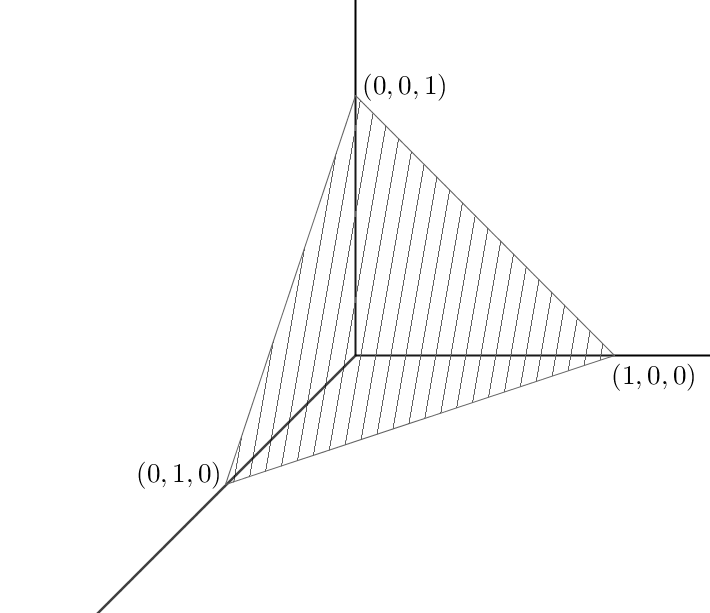
\includegraphics[height = 75mm]{molt2.png}
		\caption{Il simplesso in \(3\) dimensioni.}
		\label{fig:molt2}
	\end{centering}
\end{figure}

\begin{oss}
	Da questo esempio si deduce che
	\[
		\left(\prod_{i=1}^n x_i\right)^{\frac{1}{n}}\le\frac{1}{n}\sum_{i=1}^n x_i,
	\]
	ovvero che la media geometrica è sempre minore di quella aritmetica.
\end{oss}
%%%%%%%%%%%%%%%%%%%%%%%%%%%%%%%%%%%%%
%
%LEZIONE 08/03/2016 - TERZA SETTIMANA
%
%%%%%%%%%%%%%%%%%%%%%%%%%%%%%%%%%%%%%
%%%%%%%%%%%
%APPENDICE%
%%%%%%%%%%%
\section{Appendice}

\begin{teor}{Generalizzazioe moltiplicatori di Lagrange}{moltLagrangeGen}
	Sia \(\Omega\subset\R^n\) un aperto e sia \(f\colon \Omega\to\R\) una funzione differenziabile.
	Siano \(g_1,\dots,g_k\in C^1(\Omega,\R)\), con \(k\le n\).
	Si supponga che, preso \(x\in G=\{x\in\Omega:g_1(x)=g_2(x)=\ldots=g_k(x)=0\}\) la mappa
	\[
		\Gamma\colon\Omega\to\R^k,\Gamma(x)=
		\begin{pmatrix}
			g_1(x) \\
			\dots  \\
			g_k(x)
		\end{pmatrix}
	\]
	abbia \(\Gamma'(x)\) di rango massimo.
	Allora, se \(x_0\) è un punto di massimo o di minimo per \(f|_G\) si ha che
	\[
		\begin{cases}
			f'(x_0)=\l_1 g'_1(x_0)+\l_2 g'_2(x_0)+\dots+\l_k g'_k(x_0) \\
			g_1(x_0)=0                                                 \\
			\dots                                                      \\
			g_k(x_0)=0.
		\end{cases}
	\]
\end{teor}

\begin{proof}
	Provare per esercizio.

	Suggerimento: utilizzando Lagrange e la funzione implicita cerchiamo di esplicitare \(k\) variabili in ogni punto di \(G\) (tramite i \(k\) vincoli) in funzione delle altre \(n-k\).
\end{proof}

\begin{oss}
	Nel sistema ci sono \(n+k\) incognite, di cui \(n\) di \(x_0=(x_{0_1},\dots,x_{0_n})\) e \(k\) dei moltiplicatori di Lagrange.
	D'altronde abbiamo \(n+k\) equazioni, di cui \(k\) delle equazioni delle \(g_i\) ed \(n\) date dai gradienti.
\end{oss}

\begin{prop}{Gradiente di una funzione ortogonale alla superficie}{gradienteOrtogonale}
	Sia \(f\colon\R^n\to\R\), consideriamo la sua superficie associata
	\[
		G=\Set{\bar{x}\in\R^n | f(\bar{x})=0}.
	\]
	Allora \(\nabla f(\bar{x})\) è ortogonale a \(G\).
\end{prop}

\begin{proof}
	Basta dimostrare che presa una curva \(\g\colon[-1,1]\to G\) sulla superficie, si abbia
	\[
		\big(\g'(0),\nabla f(\bar{x})\big)=0,
	\]
	ovvero che la tangente alla curva è ortogonale al gradiente.
	Osserviamo che \(\big(f\circ\g\big)(t)\equiv 0\) in quanto \(\g\) individua solo punti di \(G\) dove \(f\) è per definizione nulla.
	Quindi
	\[
		\frac{\dd}{\dd t}\big(f\circ \g\big)(t)=0,
	\]
	inoltre, per la regola della catena
	\[
		\begin{split}
			\frac{\dd}{\dd t}\big(f\circ \g\big)(t) & =f'\big(\g(0)\big)\g'(0)\\
			& =\Big(f'\big(\g(0)\big),\g'(0)\Big)=0.\qedhere
		\end{split}
	\]
\end{proof}